{\bf Grid traversal.}
With a grid at hand, we may map the algorithmic steps from Algorithm
\ref{algorithm:dem-blueprint} onto a grid traversal.
For the traversal, we rely on a combination of a depth-first order with
space-filling curve \cite{Weinzierl:2009:Diss,Weinzierl:11:Peano}.
From a DEM point of view, the exact traversal realisation however is not that
relevant as long as the traversal is a real tree traversal, i.e.~runs through
all levels of the underlying spacetree.

\begin{figure}
  \begin{center}
    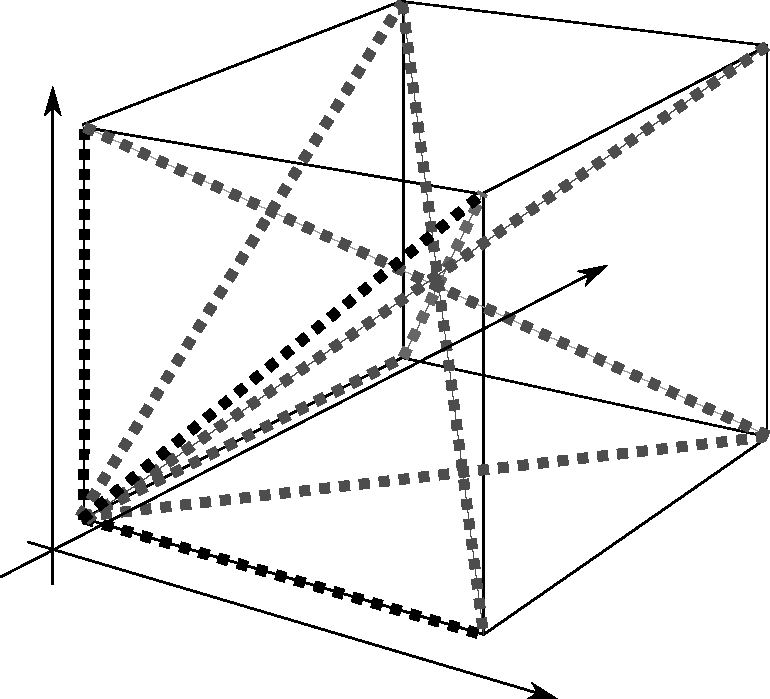
\includegraphics[width=0.25\textwidth]{sketches/collision-cube.pdf}
    \hspace{0.2cm}
    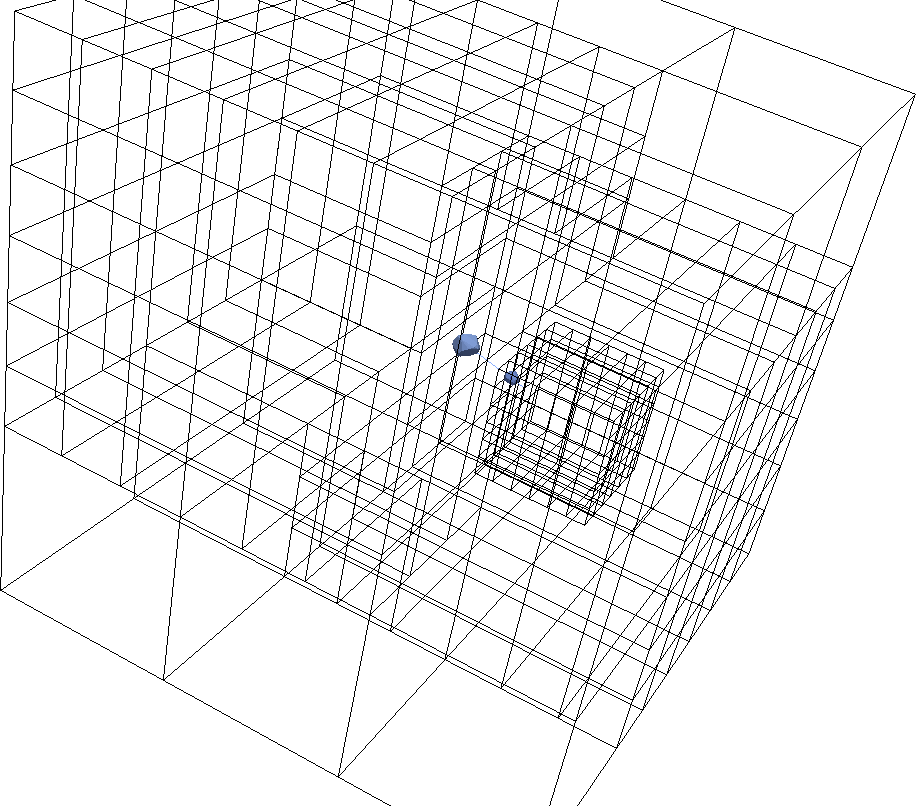
\includegraphics[width=0.3\textwidth]{experiments/two-bodies/visualisation/adaptive-grid01.png}
    \hspace{0.2cm}
    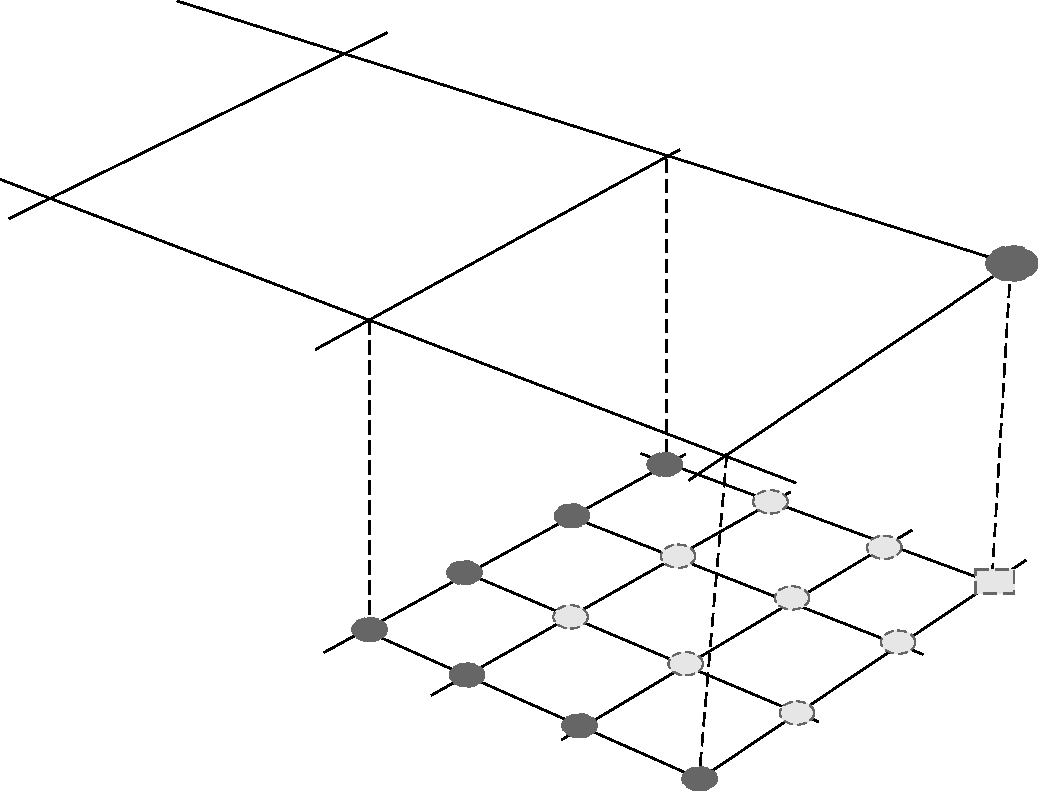
\includegraphics[width=0.3\textwidth]{sketches/multigrid.pdf}
  \end{center}
  \caption{
    Left: Whenever the grid traversal enters a cell, it checks whether particles
    assigned to one vertex do collide with particles assigned to another vertex.
    To avoid redundant collision computations, we check only some vertex pairs
    (dotted, larger lines).
    Middle: Two particles approach each other. As they are of different size,
    they might be held on different spacetree resolution levels.
    Right: In the adaptive case, particles are dropped from the coarse levels
    into the fine grid (rectangular marker) if new grid levels are added. The
    bright round vertices are children of the marked coarse grid vertex. The
    bright and the dark round markers' vertices together are the descendants of
    the marked coarse grid vertex.
  }
  \label{figure:collision-cube}
\end{figure}


We then write down the algorithm as a set of events, i.e.~we specify which
operations are performed if a vertex is read for the very first time \linebreak
(\texttt{touchVertexFirstTime}), if a cell is entered
(\texttt{enterCell}), and so forth.
Besides the actual grid hosting the particles, the grid sweeps build and
maintain two further sets of collision points (algorithm \ref{algorithm:grid-based-dem}).

\begin{algorithm}
 \caption{A grid-based DEM implementation.}
 \label{algorithm:grid-based-dem}
 \begin{algorithmic}[1]
  \Function{traverseGrid}{$\mathcal{C}$}
   \State $\mathcal{C}_{old} \gets \mathcal{C}$
   \State $\mathcal{C} \gets \emptyset$
   \While{traversal continues}
    \If{\texttt{touchVertexFirstTime}}
     \ForAll{particles $p$ associated to vertex}
      \ForAll{contact points $c \in \mathcal{C}_{old}$ associated to $p$}
       \State Update $f(p)$ through $c$
      \EndFor
      \State Update particle incl.~its triangles
     \EndFor
     \ForAll{particle pairs $(p_i,p_j)$ associated to vertex}
       \State $\mathcal{C} \gets \mathcal{C} \cup $
       \Call{findCollisions}{$p_i,p_j$}
     \EndFor
    \EndIf
    \If{\texttt{enterCell}}
     \ForAll{$2^d$ vertices adjacent to cell}
      \ForAll{particles $p$ associated to vertex}
       \If{particle should be associated to different vertex}
        \State Reassign particle
       \EndIf
      \EndFor
     \EndFor
     \ForAll{$(p_i,p_j)$ associated to different vertices (cmp.~figure)} 
      \State $\mathcal{C} \gets \mathcal{C} \cup $
       \Call{findCollisions}{$p_i,p_j$}
     \EndFor
    \EndIf
   \EndWhile
  \EndFunction

  %\Function{main}{$T$}   
  % \State $\mathcal{C} \gets \emptyset $
  % \State $t \gets 0 $
  % \For{$t < T$}
  %  \State \Call{traverseGrid}{$\mathcal{C}$}
  %  \State $t \gets t + \Delta t$
  % \EndFor
  %\EndFunction
 \end{algorithmic}
\end{algorithm} 


Our grid-based realisation is characterised by few properties:
\begin{itemize}
  \item When we load a vertex for the very first time, we make all particles
  associated to this vertex move. 
  \item When we load a vertex, we do compare all the particles associated to
  this vertex with each other and identify collision points. The comparison of
  particles associated to different vertices is realised when we enter a cell.
  Here, we do compare the vertex pairs from Figure \ref{figure:collision-cube}---left bottom
  front vertex with right bottom front vertex, all diagonal combinations, and
  so forth---such that we avoid multiple evaluations of vertex pairs. For 
  boundary cells, some special case distinctions yielding additional checks are
  added. If a cell is traversed, we assume that all its adjacent vertices are
  available, i.e.~have been read before.
  \item Whenever we run into a cell, we run through all the adjacent vertices
  and their particles. They all already have an updated position, as any vertex
  has been loaded before and thus been subject to \texttt{touchVertexFirstTime}.
  If a particle is associated to the 'wrong' vertex as it has moved and should 
  be assigned to another vertex of the cell, we do the reassignment. A particle
  may move at most one cell of its corresponding level a time.
  \item The vertex comparisons yield a set of collision points. This set is kept
  persistent for the subsequent traversal: one time step of the scheme is
  realised per two grid traversal. The amortised cost however still is one time
  step per grid traversal. This scheme picks up the idea of pipelining
  \cite{Plimpton1995}. Collision data is mapped onto the particles when we read a
  particle for the first time in the subsequent traversal. Immediately after the
  forces acting on a particle are determined, we do update the particle's
  property and also update the geometric data due to translation and rotation.
\end{itemize}

\noindent
The extension of the present scheme to multiscale trees is detailed below.
To make the algorithm correct, each contact point set between two particles does
exist twice with inverse normals.
Each set furthermore is augmented with a copy of the corresponing partner
particles' global data (mass, velocity, momentum).
Otherwise, we would have to search for this data and build up global indices,
and have to be aware that the particle's data already might have been subject to
the next time step.


\begin{observation}
The algorithm realises a single-pass policy. Geometric data is written only once
per traversal, and is read only when we read in a vertex for the first time and
when we run through a cell.
The implementation's pressure on the memory subsystem thus is minimalistic as
long as the spatial and temporal grid access locality \cite{dime} is high which
yields high cache hit rates.
We rely on a space-filling curve to
run through the grid \cite{Weinzierl:2009:Diss,Weinzierl:11:Peano} and thus
guarantee such a two-fold locality.
\end{observation}


\noindent
More sophisticated explicit schemes can be realised with the same single-touch
policy if we hold additional data per particle (acceleration, e.g.).
Such an approach picks up ideas of pipelining \cite{Plimpton1995}.
